% ============================================================
%  template.tex —— 主文件，只写内容
%  编译方式：XeLaTeX（支持中文），编译两次生成目录
% ============================================================
\documentclass[notheorems]{beamer}

\input{pptheader.tex}
\input{mycommand.tex}

\begin{document}
	
	% ============================================================
	%  元信息：修改标题、作者、单位、日期
	% ============================================================
%	\title{博士期间科研工作汇报}
%	\subtitle{基于高阶有限元的变密度拓扑优化
%		数值方法设计及其实现与应用}
	% 在 [] 中填入短标题，用于页脚显示
	\title[高阶有限元变密度拓扑优化]{基于高阶有限元的变密度拓扑优化数值方法设计及其实现与应用}
	\subtitle{博士期间科研工作汇报}
	
	% 在 [] 中填入短作者名，避免把导师信息和排版命令也带入页脚
	\author[何亮]{报告人：何亮 \\
		\vspace{5pt}
		导师：{\CJKfontspec{SimSun}魏华祎} 教授}
	
	% [] 中填入单位简称
	\institute[湘大数学院]{
		\vspace{5pt}
		湘潭大学 \\
		数学与计算科学学院
	}
	\date{\today}
	
	% ---- 封面页 ----
	\frame[plain]{\titlepage}

	
	% ============================================================
	%  个人简介页（封面与目录之间）
	% ============================================================
	{%
		\begin{frame}[plain]
			
			\begin{tikzpicture}[remember picture, overlay]
				\fill[structure.fg]
				(current page.north west)
				rectangle ([yshift=-0.077\paperheight] current page.north east);
				\node[white, anchor=west, font=\small\bfseries\sffamily]
				at ([xshift=0.025\paperwidth, yshift=-0.038\paperheight]
				current page.north west)
				{个人简介};
				\fill[panelbg]
				([yshift=-0.077\paperheight] current page.north west)
				rectangle ([xshift=0.38\paperwidth] current page.south west);
			\end{tikzpicture}
			
			\vspace{0.077\paperheight}
			
			\begin{columns}[T, totalwidth=\linewidth]
				
				% ══════════════════════════════════════════
				% 左栏：照片 + 姓名 + 研究方向
				% ══════════════════════════════════════════
				\begin{column}{0.36\linewidth}
					\vspace{0.5em}
					\begin{center}
						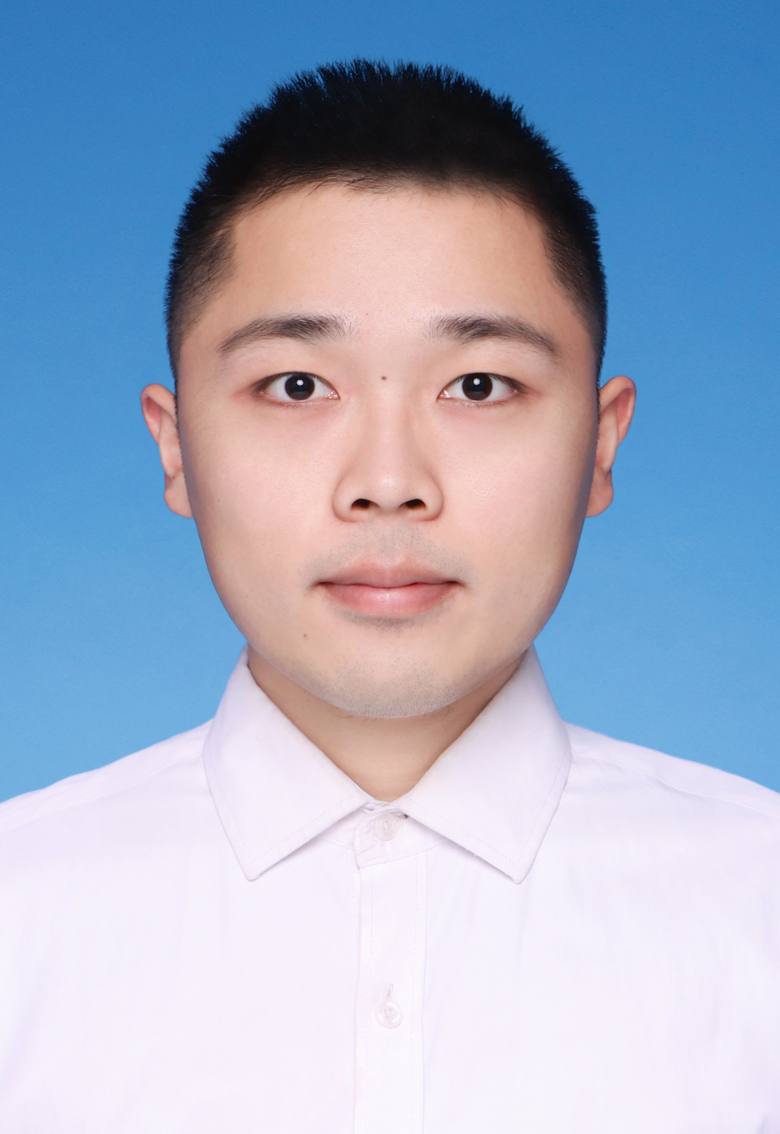
\includegraphics[width=0.50\linewidth,
						height=0.22\paperheight,
						keepaspectratio]{photo.jpg}
						
						\vspace{0.3em}
						{\fontsize{14}{18}\selectfont\bfseries\sffamily 何\quad 亮}
						
						\vspace{0.5em}
						\begin{tcolorbox}[
							colback=structure.fg, colframe=structure.fg,
							arc=4pt, boxrule=0pt,
							top=3pt, bottom=3pt, left=6pt, right=6pt,
							width=0.78\linewidth]
							\centering\color{white}\bfseries\small\sffamily 研究方向
						\end{tcolorbox}
						
						\vspace{4pt}
						% 标签：缩小字号与内边距，紧凑排列
						\tcbox[on line, arc=4pt, colback=white, colframe=tagborder,
						boxrule=0.8pt, top=1.5pt, bottom=1.5pt, left=5pt, right=5pt,
						fontupper=\footnotesize\bfseries\sffamily\color{structure.fg}]
						{偏微分方程数值方法}\\[3pt]
						\tcbox[on line, arc=4pt, colback=white, colframe=tagborder,
						boxrule=0.8pt, top=1.5pt, bottom=1.5pt, left=5pt, right=5pt,
						fontupper=\footnotesize\bfseries\sffamily\color{structure.fg}]
						{连续体结构拓扑优化}\\[3pt]
						\tcbox[on line, arc=4pt, colback=white, colframe=tagborder,
						boxrule=0.8pt, top=1.5pt, bottom=1.5pt, left=5pt, right=5pt,
						fontupper=\footnotesize\bfseries\sffamily\color{structure.fg}]
						{科学计算软件设计与实现}
					\end{center}
				\end{column}
				
				% ══════════════════════════════════════════
				% 右栏：研究主线 + 研究目标
				% ══════════════════════════════════════════
				\begin{column}{0.62\linewidth}
					\vspace{0.5em}
					
					% ── 研究主线 ────────────────────────────
					\begin{tcolorbox}[
						colback=structure.fg, colframe=structure.fg,
						arc=4pt, boxrule=0pt,
						top=3pt, bottom=3pt, left=8pt, right=8pt,
						width=\linewidth]
						\centering\color{white}\bfseries\small\sffamily 研究主线
					\end{tcolorbox}
					
					\vspace{3pt}
					{\fontsize{7.5}{10}\selectfont
						围绕基于高阶有限元的变密度拓扑优化开展系统研究，重点关注四个方面：}
					
					\vspace{4pt}
					% ── 2×2 网格 ────────────────────────────
					% 用 tabular + minipage 解决宽度与换行问题
					\begin{tabular}{@{}l@{\hspace{4pt}}l@{}}
						% 第一行
						\circnum{01}~%
						\begin{minipage}[c]{2.6cm}
							\begin{tcolorbox}[colback=panelbg!50, colframe=panelbg,
								arc=2pt, boxrule=0.5pt,
								top=2pt, bottom=2pt, left=4pt, right=4pt, nobeforeafter]
								\fontsize{7}{9}\selectfont 高阶有限元拓扑优化方法
							\end{tcolorbox}
						\end{minipage}
						&
						\circnum{03}~%
						\begin{minipage}[c]{2.6cm}
							\begin{tcolorbox}[colback=panelbg!50, colframe=panelbg,
								arc=2pt, boxrule=0.5pt,
								top=2pt, bottom=2pt, left=4pt, right=4pt, nobeforeafter]
								\fontsize{7}{9}\selectfont 胡张混合有限元拓扑优化方法
							\end{tcolorbox}
						\end{minipage}
						\\[6pt]
						% 第二行
						\circnum{02}~%
						\begin{minipage}[c]{2.6cm}
							\begin{tcolorbox}[colback=panelbg!50, colframe=panelbg,
								arc=2pt, boxrule=0.5pt,
								top=2pt, bottom=2pt, left=4pt, right=4pt, nobeforeafter]
								\fontsize{7}{9}\selectfont 多分辨率拓扑优化框架
							\end{tcolorbox}
						\end{minipage}
						&
						\circnum{04}~%
						\begin{minipage}[c]{2.6cm}
							\begin{tcolorbox}[colback=panelbg!50, colframe=panelbg,
								arc=2pt, boxrule=0.5pt,
								top=2pt, bottom=2pt, left=4pt, right=4pt, nobeforeafter]
								\fontsize{7}{9}\selectfont SOPTX 软件平台设计与实现
							\end{tcolorbox}
						\end{minipage}
					\end{tabular}
					
					\vspace{6pt}
					% ── 研究目标 ────────────────────────────
					\begin{tcolorbox}[
						colback=structure.fg, colframe=structure.fg,
						arc=4pt, boxrule=0pt,
						top=3pt, bottom=3pt, left=8pt, right=8pt,
						width=\linewidth]
						\centering\color{white}\bfseries\small\sffamily 研究目标
					\end{tcolorbox}
					
					\vspace{4pt}
					{\fontsize{8}{11}\selectfont
						面向复杂结构轻量化设计需求，围绕高精度分析、高效优化求解与软件平台实现，提升连续体结构拓扑优化的理论研究水平与工程应用能力。}
					
				\end{column}
			\end{columns}
		\end{frame}
	}%
	
	
	% ---- 每节开始自动插入目录页 ----
	\AtBeginSection[]{
		\frame<beamer>{
			\frametitle{目录}
			\tableofcontents[currentsection]
		}
	}
	
	% ---- 全局目录（可选） ----
	\begin{frame}
		\frametitle{目录}
		\tableofcontents
	\end{frame}
	
	
	% ============================================================
	\section{研究背景与关键问题}
	% ============================================================
	
	% ============================================================
	%  01-1  研究背景
	% ============================================================
	\begin{frame}
		\frametitle{研究背景}
		
		% ══════════════════════════════════════════════════════════
		%  中部图片区：三图横向并列，同宽、同高、同基线
		% ══════════════════════════════════════════════════════════
		\begin{columns}[c, totalwidth=\linewidth]
			
			\begin{column}{0.31\linewidth}
				\centering
				\begin{minipage}[c][0.40\paperheight][c]{\linewidth}
					\centering
					
\includegraphics[width=\linewidth,
					height=0.40\paperheight, keepaspectratio]{aerospace}
				\end{minipage}
				\\[4pt]
				{\small\sffamily 航空航天承力结构}
			\end{column}
			
			\begin{column}{0.31\linewidth}
				\centering
				\begin{minipage}[c][0.40\paperheight][c]{\linewidth}
					\centering
					
\includegraphics[width=\linewidth,
					height=0.40\paperheight, keepaspectratio]{building}
				\end{minipage}
				\\[4pt]
				{\small\sffamily 高层建筑抗侧力体系}
			\end{column}
			
			\begin{column}{0.31\linewidth}
				\centering
				\begin{minipage}[c][0.40\paperheight][c]{\linewidth}
					\centering
					
\includegraphics[width=\linewidth,
					height=0.40\paperheight, keepaspectratio]{biomedical}
				\end{minipage}
				\\[4pt]
				{\small\sffamily 个性化生物医疗植入体}
			\end{column}
			
		\end{columns}
		
		% ── 细分隔线（主题色调，透明度约 25%）─────────────────────
		\vspace{0.4em}
		{\color{structure.fg!25}\rule{\linewidth}{0.4pt}}
		
		% ══════════════════════════════════════════════════════════
		%  底部文字区：三条递进式结论，1/2/3 编号，左对齐
		%  采用 \makebox + \parbox 组合保证编号列与正文列精准对齐
		% ══════════════════════════════════════════════════════════
		{\fontsize{8.5}{14}\selectfont\sffamily
			\noindent
			\makebox[1.5em][l]{\textbf{1}}%
			\parbox[t]{\dimexpr\linewidth - 1.5em\relax}{%
				复杂工程结构设计对轻量化、高性能与高可靠性提出了更高要求}
			
			\vspace{5pt}\noindent
			\makebox[1.5em][l]{\textbf{2}}%
			\parbox[t]{\dimexpr\linewidth - 1.5em\relax}{%
				结构优化设计经历了由尺寸优化、形状优化到拓扑优化的递进发展}
			
			\vspace{5pt}\noindent
			\makebox[1.5em][l]{\textbf{3}}%
			\parbox[t]{\dimexpr\linewidth - 1.5em\relax}{%
				连续体结构拓扑优化直接以设计域内材料分布为设计对象，%
				是复杂结构正向设计的重要数学工具}
		}
		
	\end{frame}
	
	% ============================================================
	%  01-2  关键问题
	% ============================================================
	\begin{frame}
		\frametitle{关键问题}
		
		% ── 总述条 ───────────────────────────────────────────────
		\begin{tcolorbox}[
			colback=panelbg, colframe=structure.fg!40,
			arc=3pt, boxrule=0.5pt,
			top=3pt, bottom=3pt, left=8pt, right=8pt]
			{\fontsize{8}{12}\selectfont\sffamily
				连续体结构拓扑优化在复杂工程应用中，面临分析精度、设计分辨率、%
				复杂约束处理与统一软件实现难以兼顾的核心挑战。}
		\end{tcolorbox}
		
		\vspace{-1.2em}  % 顶部总述条与卡片之间的负间距
		
		% ── 第一行 ───────────────────────────────────────────────
		\begin{columns}[T, totalwidth=\linewidth]
			
			\begin{column}{0.485\linewidth}
				\begin{tcolorbox}[
					colback=white, colframe=structure.fg!50,
					colbacktitle=structure.fg, coltitle=white,
					fonttitle=\fontsize{8}{10}\selectfont\bfseries\sffamily,
					title={\circnum{01}\enspace 低阶有限元分析精度受限},
					arc=3pt, boxrule=0.5pt,
					toptitle=0.25pt, bottomtitle=0.25pt,
					top=3pt, bottom=3pt, left=6pt, right=6pt]
					{\fontsize{7.5}{11}\selectfont\sffamily
						\begin{itemize}
							\setlength{\itemsep}{1pt}
							\setlength{\topsep}{1pt}
							\setlength{\parsep}{0pt}
							\setlength{\parskip}{0pt}
							\item 复杂变形与局部应力场分析中，传统低阶有限元精度受限
							\item 难以为拓扑优化提供高质量物理响应信息
					\end{itemize}}
				\end{tcolorbox}
			\end{column}
			
			\begin{column}{0.485\linewidth}
				\begin{tcolorbox}[
					colback=white, colframe=structure.fg!50,
					colbacktitle=structure.fg, coltitle=white,
					fonttitle=\fontsize{8}{10}\selectfont\bfseries\sffamily,
					title={\circnum{02}\enspace 分辨率与规模难以兼顾},
					arc=3pt, boxrule=0.5pt,
					toptitle=0.25pt, bottomtitle=0.25pt,
					top=3pt, bottom=3pt, left=6pt, right=6pt]
					{\fontsize{7.5}{11}\selectfont\sffamily
						\begin{itemize}
							\setlength{\itemsep}{1pt}
							\setlength{\topsep}{1pt}
							\setlength{\parsep}{0pt}
							\setlength{\parskip}{0pt}
							\item 高分辨率设计有助于获得边界清晰、细节丰富的优化构型
							\item 单分辨率框架下，高分辨率常伴随计算规模显著增长
					\end{itemize}}
				\end{tcolorbox}
			\end{column}
			
		\end{columns}
		
		\vspace{0.2em}  % 两行卡片之间的固定间距
		
		% ── 第二行 ───────────────────────────────────────────────
		\begin{columns}[T, totalwidth=\linewidth]
			
			\begin{column}{0.485\linewidth}
				\begin{tcolorbox}[
					colback=white, colframe=structure.fg!50,
					colbacktitle=structure.fg, coltitle=white,
					fonttitle=\fontsize{8}{10}\selectfont\bfseries\sffamily,
					title={\circnum{03}\enspace 复杂局部约束求解困难},
					arc=3pt, boxrule=0.5pt,
					toptitle=0.25pt, bottomtitle=0.25pt,
					top=3pt, bottom=3pt, left=6pt, right=6pt]
					{\fontsize{7.5}{11}\selectfont\sffamily
						\begin{itemize}
							\setlength{\itemsep}{1pt}
							\setlength{\topsep}{1pt}
							\setlength{\parsep}{0pt}
							\setlength{\parskip}{0pt}
							\item 局部应力约束存在应力奇异性，约束建模与求解较为困难
							\item 大量局部约束易导致求解困难与演化不稳定
					\end{itemize}}
				\end{tcolorbox}
			\end{column}
			
			\begin{column}{0.485\linewidth}
				\begin{tcolorbox}[
					colback=white, colframe=structure.fg!50,
					colbacktitle=structure.fg, coltitle=white,
					fonttitle=\fontsize{8}{10}\selectfont\bfseries\sffamily,
					title={\circnum{04}\enspace 缺乏统一软件实现框架},
					arc=3pt, boxrule=0.5pt,
					toptitle=0.25pt, bottomtitle=0.25pt,
					top=3pt, bottom=3pt, left=6pt, right=6pt]
					{\fontsize{7.5}{11}\selectfont\sffamily
						\begin{itemize}
							\setlength{\itemsep}{1pt}
							\setlength{\topsep}{1pt}
							\setlength{\parsep}{0pt}
							\setlength{\parskip}{0pt}
							\item 先进数值方法与高性能计算机制缺乏统一组织与实现框架
							\item 自动微分、多后端与异构计算支持仍显不足
					\end{itemize}}
				\end{tcolorbox}
			\end{column}
			
		\end{columns}
		
	\end{frame}
	
	% ============================================================
	\section{主要研究工作}
	% ============================================================
	
	% ============================================================
	%  02-1  主要研究工作概览
	% ============================================================
	\begin{frame}
		\frametitle{主要研究工作概览}
		
		\begin{tcolorbox}[
			colback=panelbg, colframe=structure.fg!40,
			arc=3pt, boxrule=0.5pt,
			top=2pt, bottom=2pt, left=8pt, right=8pt]
			{\fontsize{7.5}{11}\selectfont\sffamily
				围绕连续体结构拓扑优化中的分析精度、分辨率提升与复杂约束处理问题，%
				系统开展了三类高精度数值方法研究。}
		\end{tcolorbox}
		
		\vspace{-1.5em}  % 顶部总述条与卡片之间的负间距
		
		\begin{columns}[T, totalwidth=\linewidth]
			
			% ── 卡片 01 ──────────────────────────────────────────────
			\begin{column}{0.318\linewidth}
				\begin{tcolorbox}[
					colback=white, colframe=structure.fg!50,
					colbacktitle=structure.fg, coltitle=white,
					fonttitle=\fontsize{7}{9.5}\selectfont\bfseries\sffamily,
					title={\circnum{01}\enspace 任意次拉格朗日有限元拓扑优化方法},
					arc=3pt, boxrule=0.5pt,
					toptitle=1pt, bottomtitle=1pt,
					top=4pt, bottom=4pt, left=5pt, right=5pt,
					height=0.53\paperheight, valign=top]
					\setlength{\parskip}{0pt}%
					\sloppy
					\noindent
					\tcbox[on line, arc=2pt,
					colback=structure.fg!15, colframe=structure.fg!15,
					boxrule=0pt, top=1pt, bottom=1pt, left=2pt, right=2pt,
					fontupper=\fontsize{6}{7.5}\selectfont\bfseries\sffamily\color{structure.fg}
					]{针对问题}\enspace
					{\fontsize{7.5}{11}\selectfont\sffamily 提升位移场与灵敏度分析精度}
					\par\vspace{5pt}%
					\noindent
					\tcbox[on line, arc=2pt,
					colback=structure.fg!15, colframe=structure.fg!15,
					boxrule=0pt, top=1pt, bottom=1pt, left=2pt, right=2pt,
					fontupper=\fontsize{6}{7.5}\selectfont\bfseries\sffamily\color{structure.fg}
					]{核心思路}\enspace
					{\fontsize{7.5}{11}\selectfont\sffamily
						系统比较不同单元类型、不同离散阶次及不同设计变量表征下的拓扑优化表现，%
						分析高阶离散的适用特征与精度优势}
				\end{tcolorbox}
			\end{column}
			
			% ── 卡片 02 ──────────────────────────────────────────────
			\begin{column}{0.318\linewidth}
				\begin{tcolorbox}[
					colback=white, colframe=structure.fg!50,
					colbacktitle=structure.fg, coltitle=white,
					fonttitle=\fontsize{7}{9.5}\selectfont\bfseries\sffamily,
					title={\circnum{02}\enspace 基于高阶有限元的多分辨率拓扑优化框架},
					arc=3pt, boxrule=0.5pt,
					toptitle=1pt, bottomtitle=1pt,
					top=4pt, bottom=4pt, left=5pt, right=5pt,
					height=0.53\paperheight, valign=top]
					\setlength{\parskip}{0pt}%
					\sloppy
					\noindent
					\tcbox[on line, arc=2pt,
					colback=structure.fg!15, colframe=structure.fg!15,
					boxrule=0pt, top=1pt, bottom=1pt, left=2pt, right=2pt,
					fontupper=\fontsize{6}{7.5}\selectfont\bfseries\sffamily\color{structure.fg}
					]{针对问题}\enspace
					{\fontsize{7.5}{11}\selectfont\sffamily 缓解高精度分析与高分辨率设计之间的矛盾}
					\par\vspace{5pt}%
					\noindent
					\tcbox[on line, arc=2pt,
					colback=structure.fg!15, colframe=structure.fg!15,
					boxrule=0pt, top=1pt, bottom=1pt, left=2pt, right=2pt,
					fontupper=\fontsize{6}{7.5}\selectfont\bfseries\sffamily\color{structure.fg}
					]{核心思路}\enspace
					{\fontsize{7.5}{11}\selectfont\sffamily
						构建设计网格、分析网格与密度积分网格相互独立的多分辨率框架，%
						兼顾分析精度与拓扑表达分辨率}
				\end{tcolorbox}
			\end{column}
			
			% ── 卡片 03 ──────────────────────────────────────────────
			\begin{column}{0.318\linewidth}
				\begin{tcolorbox}[
					colback=white, colframe=structure.fg!50,
					colbacktitle=structure.fg, coltitle=white,
					fonttitle=\fontsize{7}{9.5}\selectfont\bfseries\sffamily,
					title={\circnum{03}\enspace 任意次胡张混合有限元拓扑优化方法},
					arc=3pt, boxrule=0.5pt,
					toptitle=1pt, bottomtitle=1pt,
					top=4pt, bottom=4pt, left=5pt, right=5pt,
					height=0.53\paperheight, valign=top]
					\setlength{\parskip}{0pt}%
					\sloppy
					\noindent
					\tcbox[on line, arc=2pt,
					colback=structure.fg!15, colframe=structure.fg!15,
					boxrule=0pt, top=1pt, bottom=1pt, left=2pt, right=2pt,
					fontupper=\fontsize{6}{7.5}\selectfont\bfseries\sffamily\color{structure.fg}
					]{针对问题}\enspace
					{\fontsize{7.5}{11}\selectfont\sffamily
						提升近不可压缩材料与局部应力约束问题的求解可靠性}
					\par\vspace{5pt}%
					\noindent
					\tcbox[on line, arc=2pt,
					colback=structure.fg!15, colframe=structure.fg!15,
					boxrule=0pt, top=1pt, bottom=1pt, left=2pt, right=2pt,
					fontupper=\fontsize{6}{7.5}\selectfont\bfseries\sffamily\color{structure.fg}
					]{核心思路}\enspace
					{\fontsize{7.5}{11}\selectfont\sffamily
						基于任意次胡张混合有限元，构建高精度应力—位移混合离散与优化求解方法}
				\end{tcolorbox}
			\end{column}
			
		\end{columns}
	
		% ── 底部总结条 ──────────────────────────────────────────────
		\begin{tcolorbox}[
			colback=structure.fg, colframe=structure.fg,
			arc=3pt, boxrule=0pt,
			top=3pt, bottom=3pt, left=8pt, right=8pt]
			{\fontsize{7.5}{11}\selectfont\sffamily\color{white}
				上述研究形成了从高阶位移离散到多分辨率解耦，再到高精度混合建模的系统方法链条。}
		\end{tcolorbox}
		
	\end{frame}
	
	% ============================================================
	%  02-2  研究动机与核心思路
	% ============================================================
	\begin{frame}
		\frametitle{任意次拉格朗日有限元拓扑优化方法}
		
		% ── 顶部总述条 ──────────────────────────────────────────────
		\begin{tcolorbox}[
			colback=panelbg, colframe=structure.fg!40,
			arc=3pt, boxrule=0.5pt,
			top=2pt, bottom=2pt, left=8pt, right=8pt]
			{\fontsize{7.5}{11}\selectfont\sffamily
				现有变密度拓扑优化多基于低阶位移有限元实现，而高阶拉格朗日有限元在分析精度与%
				边界表达方面具有潜力，其在不同离散设置下对拓扑优化结果的影响规律仍有待系统研究。}
		\end{tcolorbox}
		
		\vspace{-1.5em}  % 顶部总述条与卡片之间的负间距
		
		% ── 左右两栏卡片 ────────────────────────────────────────────
		\begin{columns}[T, totalwidth=\linewidth]
			
			% ── 左栏：研究动机 ───────────────────────────────────────
			\begin{column}{0.485\linewidth}
				\begin{tcolorbox}[
					colback=white, colframe=structure.fg!50,
					colbacktitle=structure.fg, coltitle=white,
					fonttitle=\fontsize{8}{10}\selectfont\bfseries\sffamily,
					title={\circnum{01}\enspace 研究动机},
					arc=3pt, boxrule=0.5pt,
					toptitle=0.25pt, bottomtitle=0.25pt,
					top=3pt, bottom=3pt, left=6pt, right=6pt,
					height=0.48\paperheight, valign=top]
					{\fontsize{7.5}{11}\selectfont\sffamily
						\begin{itemize}
							\setlength{\itemsep}{3pt}
							\setlength{\topsep}{1pt}
							\setlength{\parsep}{0pt}
							\setlength{\parskip}{0pt}
							\item 传统实现多依赖低阶位移有限元，复杂结构响应的分析精度仍受限制
							\item 高阶拉格朗日有限元具有更强逼近能力，但其优势与适用条件尚不清晰
							\item 需要在统一框架下系统比较不同离散设置对拓扑优化结果的影响规律
					\end{itemize}}
				\end{tcolorbox}
			\end{column}
			
			% ── 右栏：核心思路 ───────────────────────────────────────
			\begin{column}{0.485\linewidth}
				\begin{tcolorbox}[
					colback=white, colframe=structure.fg!50,
					colbacktitle=structure.fg, coltitle=white,
					fonttitle=\fontsize{8}{10}\selectfont\bfseries\sffamily,
					title={\circnum{02}\enspace 核心思路},
					arc=3pt, boxrule=0.5pt,
					toptitle=0.25pt, bottomtitle=0.25pt,
					top=3pt, bottom=3pt, left=6pt, right=6pt,
					height=0.48\paperheight, valign=top]
					{\fontsize{7.5}{11}\selectfont\sffamily
						\setlength{\tabcolsep}{4pt}%
						\begin{tabular}{@{}r@{\hspace{4pt}}p{0.62\linewidth}@{}}
							\textbf{比较对象：} & 单元类型、离散阶次与设计变量表征 \\[4pt]
							\textbf{具体设置：} & 单纯形/张量积单元，任意次拉格朗日有限元，单元密度/节点密度 \\[4pt]
							\textbf{统一原则：} & 在统一物理长度尺度与求解参数下开展比较 \\[4pt]
							\textbf{比较指标：} & 拓扑构型、分析精度与计算性能 \\
					\end{tabular}}
				\end{tcolorbox}
			\end{column}
			
		\end{columns}
		
		% ── 底部强调条 ──────────────────────────────────────────────
		\begin{tcolorbox}[
			colback=structure.fg, colframe=structure.fg,
			arc=3pt, boxrule=0pt,
			top=3pt, bottom=3pt, left=8pt, right=8pt]
			{\fontsize{7.5}{11}\selectfont\sffamily\color{white}
				揭示高阶拉格朗日有限元在典型变密度拓扑优化中的适用特征、精度优势及局限性。}
		\end{tcolorbox}
		
	\end{frame}
	
	% ============================================================
	%  02-3  比较研究结论
	% ============================================================
	\begin{frame}
		\frametitle{任意次拉格朗日有限元拓扑优化方法}
		
		% ── 顶部总述条 ──────────────────────────────────────────────
		\begin{tcolorbox}[
			colback=panelbg, colframe=structure.fg!40,
			arc=3pt, boxrule=0.5pt,
			top=2pt, bottom=2pt, left=8pt, right=8pt]
			{\fontsize{7.5}{11}\selectfont\sffamily
				系统比较表明，高阶拉格朗日有限元能够提升物理响应评估质量，但其优势发挥受%
				设计变量表征、显式正则化及单分辨率耦合框架的共同影响。}
		\end{tcolorbox}
		
		\vspace{-1.5em}  % 顶部总述条与卡片之间的负间距
		
		% ── 三列结论卡片 ────────────────────────────────────────────
		\begin{columns}[T, totalwidth=\linewidth]
			
			% ── 卡片 01 ──────────────────────────────────────────────
			\begin{column}{0.318\linewidth}
				\begin{tcolorbox}[
					colback=white, colframe=structure.fg!50,
					colbacktitle=structure.fg, coltitle=white,
					fonttitle=\fontsize{7}{9.5}\selectfont\bfseries\sffamily,
					title={\circnum{01}\enspace 高阶有限元的优势与局限},
					arc=3pt, boxrule=0.5pt,
					toptitle=1pt, bottomtitle=1pt,
					top=4pt, bottom=4pt, left=5pt, right=5pt,
					height=0.44\paperheight, valign=top]
					\setlength{\parskip}{0pt}%
					\sloppy
					{\fontsize{7.5}{11}\selectfont\sffamily
						高阶有限元能够改善物理状态评估质量，消除低阶离散引起的虚假刚度；%
						但单纯提升插值阶次并不能替代显式正则化，且会增加计算成本。}
				\end{tcolorbox}
			\end{column}
			
			% ── 卡片 02 ──────────────────────────────────────────────
			\begin{column}{0.318\linewidth}
				\begin{tcolorbox}[
					colback=white, colframe=structure.fg!50,
					colbacktitle=structure.fg, coltitle=white,
					fonttitle=\fontsize{7}{9.5}\selectfont\bfseries\sffamily,
					title={\circnum{02}\enspace 不同设计变量表征的差异},
					arc=3pt, boxrule=0.5pt,
					toptitle=1pt, bottomtitle=1pt,
					top=4pt, bottom=4pt, left=5pt, right=5pt,
					height=0.44\paperheight, valign=top]
					\setlength{\parskip}{0pt}%
					\sloppy
					{\fontsize{7.5}{11}\selectfont\sffamily
						单元密度表征形式直接、收敛高效，但边界易呈阶梯状；%
						节点密度表征边界过渡更平滑，但在某些设置下可能出现准收敛现象，%
						导致计算代价上升。}
				\end{tcolorbox}
			\end{column}
			
			% ── 卡片 03 ──────────────────────────────────────────────
			\begin{column}{0.318\linewidth}
				\begin{tcolorbox}[
					colback=white, colframe=structure.fg!50,
					colbacktitle=structure.fg, coltitle=white,
					fonttitle=\fontsize{7}{9.5}\selectfont\bfseries\sffamily,
					title={\circnum{03}\enspace 单分辨率框架下高阶优势受限},
					arc=3pt, boxrule=0.5pt,
					toptitle=1pt, bottomtitle=1pt,
					top=4pt, bottom=4pt, left=5pt, right=5pt,
					height=0.44\paperheight, valign=top]
					\setlength{\parskip}{0pt}%
					\sloppy
					{\fontsize{7.5}{11}\selectfont\sffamily
						在统一物理半径的显式正则化作用下，不同方案往往收敛到一致的宏观构型；%
						单纯提升离散阶次并未带来实质性的拓扑改进，高阶有限元的精度优势难以充分释放。}
				\end{tcolorbox}
			\end{column}
			
		\end{columns}
		
		% ── 底部过渡条 ──────────────────────────────────────────────
		\begin{tcolorbox}[
			colback=structure.fg, colframe=structure.fg,
			arc=3pt, boxrule=0pt,
			top=3pt, bottom=3pt, left=8pt, right=8pt]
			{\fontsize{7.5}{11}\selectfont\sffamily\color{white}
				上述结果表明，单纯提升有限元阶次难以同时兼顾高精度分析与高分辨率拓扑表达，%
				这直接引出了后续的多分辨率拓扑优化研究。}
		\end{tcolorbox}
		
	\end{frame}
	
	% ============================================================
	%  02-4  无过滤/弱正则化结果：高阶分析更真实，但成本更高
	% ============================================================
	\begin{frame}
		\frametitle{高阶有限元的优势与局限}
		
		% ── 顶部总述条 ──────────────────────────────────────────────
		\begin{tcolorbox}[
			colback=panelbg, colframe=structure.fg!40,
			arc=3pt, boxrule=0.5pt,
			top=2pt, bottom=2pt, left=8pt, right=8pt]
			{\fontsize{7.5}{11}\selectfont\sffamily
				高阶有限元主要提升物理响应评估质量；随阶次提高，低阶离散引起的虚假刚度与局部振荡明显减弱，%
				棋盘格现象在一定程度上得到削弱，结构分析结果更接近真实物理水平。}
		\end{tcolorbox}
		
		\vspace{-1.0em}
		
		% ── 主体：左图 + 右侧两框 ───────────────────────────────────
		\begin{columns}[T, totalwidth=\linewidth]
			
			% ── 左栏：k=1 与 k=4 两图 ────────────────────────────────
			\begin{column}{0.55\linewidth}
				\begin{tcolorbox}[
					colback=white, colframe=structure.fg!40,
					arc=3pt, boxrule=0.5pt,
					top=4pt, bottom=4pt, left=4pt, right=4pt,
					valign=top]
					
					% 公共说明（只写一次）
					{\centering\fontsize{7}{9}\selectfont\sffamily\color{structure.fg}
						MBB 梁，无过滤，单元密度表征\par}
					
					\vspace{5pt}
					
					% k=1
					\centering
					
\includegraphics[width=0.88\linewidth,
					height=0.115\paperheight, keepaspectratio]{mbb_nofilter_k1}
					\\[3pt]
					{\fontsize{7.5}{10}\selectfont\sffamily $k=1,c=203.07$}
					
					\vspace{-4pt}
					{\color{structure.fg!20}\rule{0.88\linewidth}{0.4pt}}
					\vspace{8pt}
					
					% k=4
					
\includegraphics[width=0.88\linewidth,
					height=0.115\paperheight, keepaspectratio]{mbb_nofilter_k4}
					\\[3pt]
					{\fontsize{7.5}{10}\selectfont\sffamily $k=4,c=218.66$}
					
				\end{tcolorbox}
			\end{column}
			
			% ── 右栏：两个结论框 ──────────────────────────────────────
			\begin{column}{0.43\linewidth}
				
				\begin{tcolorbox}[
					colback=white, colframe=structure.fg!50,
					colbacktitle=structure.fg, coltitle=white,
					fonttitle=\fontsize{7.5}{10}\selectfont\bfseries\sffamily,
					title={\circnum{01}\enspace 削弱虚假刚度，提升分析真实性},
					arc=3pt, boxrule=0.5pt,
					toptitle=1pt, bottomtitle=1pt,
					top=5pt, bottom=5pt, left=6pt, right=6pt]
					\setlength{\parskip}{0pt}\sloppy
					{\fontsize{7.5}{11}\selectfont\sffamily
						升阶后，低阶离散引入的虚假刚度减弱，目标函数评估更接近真实物理响应。}
				\end{tcolorbox}
				
				\vspace{4pt}
				
				\begin{tcolorbox}[
					colback=white, colframe=structure.fg!50,
					colbacktitle=structure.fg, coltitle=white,
					fonttitle=\fontsize{7.5}{10}\selectfont\bfseries\sffamily,
					title={\circnum{02}\enspace 局部振荡减弱，构型更平顺},
					arc=3pt, boxrule=0.5pt,
					toptitle=1pt, bottomtitle=1pt,
					top=5pt, bottom=5pt, left=6pt, right=6pt]
					\setlength{\parskip}{0pt}\sloppy
					{\fontsize{7.5}{11}\selectfont\sffamily
						阶次提高，密度场中的局部细碎振荡减弱，材料分布更连贯，构型表达更平顺。}
				\end{tcolorbox}
				
			\end{column}
			
		\end{columns}
		
		% ── 底部过渡条 ──────────────────────────────────────────────
		\begin{tcolorbox}[
			colback=structure.fg, colframe=structure.fg,
			arc=3pt, boxrule=0pt,
			top=3pt, bottom=3pt, left=8pt, right=8pt]
			{\fontsize{7.5}{11}\selectfont\sffamily\color{white}
				\textbf{局限：}高阶有限元改善的是分析质量而非正则化机制，%
				且计算规模随阶次提升而显著增长。}
		\end{tcolorbox}
		
	\end{frame}
	
	% 【普通帧】文字 + 列表
	\begin{frame}
		\frametitle{帧标题}
		正文内容写在这里。
		\begin{itemize}
			\item 要点一；
			\item 要点二；
			\item \highlightit{需要高亮的结论}。
		\end{itemize}
	\end{frame}
	
	% 【公式帧】
	\begin{frame}
		\frametitle{公式帧}
		考虑以下方程：
		$$
		\left\{
		\begin{aligned}
			-\Delta u &= f \quad \text{in} \quad \Omega, \\
			u         &= 0 \quad \text{on} \quad \partial\Omega.
		\end{aligned}
		\right.
		$$
	\end{frame}
	
	% 【逐步显示帧】\uncover
	\begin{frame}
		\frametitle{逐步显示帧}
		\uncover<1->{
			\begin{itemize}
				\item 第一步显示的内容；
			\end{itemize}
		}
		\uncover<2->{
			\begin{itemize}
				\item 第二步显示的内容；
			\end{itemize}
			\centering\highlightit{点击后出现的重要结论。}
		}
	\end{frame}
	
	% 【分栏帧】左文字 + 右图
	\begin{frame}
		\frametitle{左右分栏帧}
		\begin{minipage}[b]{0.55\linewidth}
			\begin{itemize}
				\item 左侧文字说明；
				\item 右侧放图片。
			\end{itemize}
		\end{minipage}
		\hfill
		\begin{minipage}[b]{0.38\linewidth}
			\centering
			% 替换为实际图片路径，例如：
			% \includegraphics[width=\textwidth]{../figures/example.pdf}
		\end{minipage}
	\end{frame}
	
	% 【定理帧】
	\begin{frame}
		\frametitle{定理帧}
		\begin{lemma}[引理名称]
			引理内容。
		\end{lemma}
		\begin{theorem}[定理名称]
			$$
			|u - u_h|_m \lesssim h^{k+1-m} |u|_{k+1}.
			$$
		\end{theorem}
	\end{frame}
	
	% 【\only 切换帧】同位置切换不同内容（常用于误差表格对比）
	\begin{frame}
		\frametitle{\texttt{\textbackslash only} 切换帧}
		\only<1>{
			\begin{table}
				\centering
				\caption{误差表}
				\begin{tabular}{|c|c|c|}
					\hline
					$h$ & 误差 & 阶数 \\ \hline
					0.1  & 1.2e-2 & --   \\ \hline
					0.05 & 3.1e-3 & 1.95 \\ \hline
				\end{tabular}
			\end{table}
		}
		\only<2>{
			\begin{table}
				\centering
				\caption{计算时间对比}
				\begin{tabular}{|c|c|c|}
					\hline
					$h$ & 方法一 (s) & 方法二 (s) \\ \hline
					0.1  & 0.31 & 0.14 \\ \hline
					0.05 & 0.88 & 0.25 \\ \hline
				\end{tabular}
			\end{table}
		}
	\end{frame}
	
	\begin{frame}
		\frametitle{帧标题}
		内容。
	\end{frame}
	
	% ============================================================
	%  结束页
	% ============================================================
	\begin{frame}
		\centering{\huge 感谢聆听，期待您的批评指正！}
	\end{frame}
	
	
	% ============================================================
	\section{软件平台开发}
	% ============================================================
	
	
	% ============================================================
	\section{代表性成果与项目}
	% ============================================================
	
	% ============================================================
	\section{未来工作安排}
	% ============================================================
	
	
\end{document}